\documentclass{beamer}
\usepackage{beamerthemesplit}
\usepackage[T1]{fontenc}
\usepackage[austrian]{babel}
\usepackage[utf8]{inputenc}
\usepackage{amsmath}
\usepackage{subfig}
\usepackage{listings}
\lstset{
  basicstyle=\ttfamily,
  mathescape
}

\title{Erzeugung von Gebirgsketten}
\author{Bernhard Fritz}
\date{01. Dezember 2015}
\logo{
\includegraphics[height=1.5cm]{../Bilder/Uni_Logo_4C.pdf}}

\makeatletter
       \newcount\c@p
       \newcount\c@m
              \newcount\c@pp
       \newcount\c@mm
\def\insertsectionnavigation#1{%
  \hbox to #1{%
    \vbox{{\usebeamerfont{section in head/foot}\usebeamercolor[fg]{section in head/foot}%
     \vskip0.5625ex%
    \def\slideentry##1##2##3##4##5##6{}%
     \def\sectionentry##1##2##3##4##5{%
       \ifnum##5=\c@part%
       \def\insertsectionhead{##2}%
       \def\insertsectionheadnumber{##1}%
       \def\insertpartheadnumber{##5}%
       \c@p=\c@section%
       \c@m=\c@section%
      \c@pp=\c@section%
       \c@mm=\c@section%
       \advance\c@m by -1 %
       \advance\c@p by 1 %
       \advance\c@mm by -2 %
       \advance\c@pp by 2 %
       %
       \ifnum \c@section=1
                    \ifnum\c@section=##1%
               \setbox\beamer@tempbox=\hbox{%
              \hyperlink{Navigation##3}{\hbox to #1{%
             {\hskip0.3cm\usebeamertemplate{section in head/foot}\hskip0.3cm}}}}%
             \else%
                 \ifnum##1=\c@p%
                 \setbox\beamer@tempbox=\hbox{%
                  \hyperlink{Navigation##3}{\hbox to #1{%
                 {\hskip0.3cm\usebeamertemplate{section in head/foot shaded}\hskip0.3cm}}}}
                 %
                \else%
                 \ifnum##1=\c@pp%
                 \setbox\beamer@tempbox=\hbox{%
                  \hyperlink{Navigation##3}{\hbox to #1{%
               {\hskip0.3cm\usebeamertemplate{section in head/foot shaded}\hskip0.3cm}}}}%
               %
               \else%
               %
               \fi%
               \fi%
               %
            \fi%%
         \else%
  \ifnum \c@section=\beamer@sectionmax
               \ifnum\c@section=##1%
               \setbox\beamer@tempbox=\hbox{%
              \hyperlink{Navigation##3}{\hbox to #1{%
             {\hskip0.3cm\usebeamertemplate{section in head/foot}\hskip0.3cm}}}}%
             \else%
                 \ifnum##1=\c@m%
                 \setbox\beamer@tempbox=\hbox{%
                  \hyperlink{Navigation##3}{\hbox to #1{%
                 {\hskip0.3cm\usebeamertemplate{section in head/foot shaded}\hskip0.3cm}}}}
                 %
                \else%
                 \ifnum##1=\c@mm%
                 \setbox\beamer@tempbox=\hbox{%
                  \hyperlink{Navigation##3}{\hbox to #1{%
               {\hskip0.3cm\usebeamertemplate{section in head/foot shaded}\hskip0.3cm}}}}%
               %
               \else%
               %
               \fi%
               \fi%
               %
            \fi%%
       \else%
             \ifnum\c@section=##1%
               \setbox\beamer@tempbox=\hbox{%
              \hyperlink{Navigation##3}{\hbox to #1{%
             {\hskip0.3cm\usebeamertemplate{section in head/foot}\hskip0.3cm}}}}%
             \else%
                 \ifnum##1=\c@m%
                 \setbox\beamer@tempbox=\hbox{%
                  \hyperlink{Navigation##3}{\hbox to #1{%
                 {\hskip0.3cm\usebeamertemplate{section in head/foot shaded}\hskip0.3cm}}}}
                 %
                \else%
                 \ifnum##1=\c@p%
                 \setbox\beamer@tempbox=\hbox{%
                  \hyperlink{Navigation##3}{\hbox to #1{%
               {\hskip0.3cm\usebeamertemplate{section in head/foot shaded}\hskip0.3cm}}}}%
               %
               \else%
               %
               \fi%
               \fi%
               %
            \fi%%
            %
            \fi
            \fi
            %

      \ht\beamer@tempbox=1.6875ex%
       \dp\beamer@tempbox=0.75ex%
       \box\beamer@tempbox\fi}%
     \dohead\vskip0.5625ex}}\hfil}}


\setbeamertemplate{headline}%{split theme} % full manual adjustment
{%
  \leavevmode%
  \@tempdimb=3em%
  \ifdim\@tempdimb>0pt%
    \advance\@tempdimb by 1.825ex%
    \begin{beamercolorbox}[wd=.5\paperwidth,ht=\@tempdimb]{section in head/foot}%
      \vbox to\@tempdimb{\vfil\insertsectionnavigation{.5\paperwidth}\vfil}%
    \end{beamercolorbox}%
    \begin{beamercolorbox}[wd=.5\paperwidth,ht=\@tempdimb]{subsection in head/foot}%
      \vbox to\@tempdimb{\vfil\insertsubsectionnavigation{.5\paperwidth}\vfil}%
    \end{beamercolorbox}%
  \fi%
}



\makeatother

\setbeamertemplate{navigation symbols}{}%remove navigation symbols

\setbeamertemplate{caption}{\raggedright\insertcaption\par}
\captionsetup[subfigure]{labelformat=empty}

\begin{document}

  \frame{\titlepage}

  \section*{Überblick}
  \frame{
    \frametitle{Überblick}
    \tableofcontents
  }

  \section{Problembeschreibung}

  \frame{
    \frametitle{Problembeschreibung}
    \begin{itemize}
      \item Das von Kamal und Sarwar veröffentlichte Paper ``Parametrically Controlled Terrain Generation'' stellt einen Algorithmus zur Generierung eines einzelnen Berges vor
      \item Ziel ist es den vorgeschlagenen Algorithmus zu erweitern um es zu ermöglichen ganze Gebirgsketten kontrolliert generieren zu können
    \end{itemize}
  }

  \section{Methoden zur Erzeugung von Gebirgen}

  \frame{
    \frametitle{Erzeugen von Gebirgen mithilfe von Höhenkarten}
    \begin{itemize}
      \item Schwarz-weiß Bild als Datenträger
      \item 1 Byte pro Pixel bedeutet 256 mögliche Höhenabstufungen
      \item \( h = f(x,y) \)
      \begin{figure}[t]
        \subfloat[Kamal, Sarwar]{%
          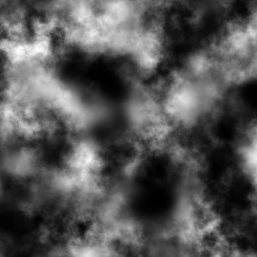
\includegraphics[height=3cm]{../Bilder/heightmap.png}
        }
        \hspace{1cm}
        \subfloat[Kamal, Sarwar]{%
          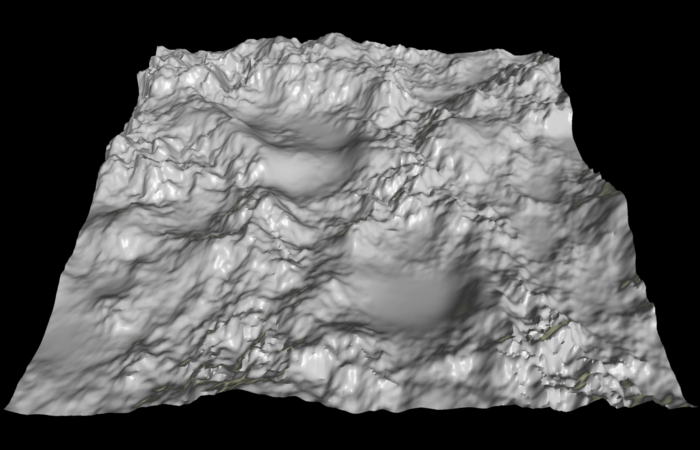
\includegraphics[height=3cm]{../Bilder/heightmap_rendered.png}
        }
      \end{figure}
    \end{itemize}
  }

\begin{frame}[fragile]
\frametitle{Erzeugen von Gebirgen mithilfe von Algorithmen}
\begin{itemize}
\item<1->{\only<2-5>{\color{blue}} Midpoint displacement / Diamond-square Algorithm}
\begin{onlyenv}<2-5>
\begin{footnotesize}
\begin{verbatim}
Wiederhole solange Segmente nicht zu klein:
  Für jedes Segment:
    Teile das Segment in der Mitte
    Erhöhe den Mittelpunkt um x aus [-R, R]
  Halbiere R
\end{verbatim}
\end{footnotesize}
\end{onlyenv}
\item<1->{\only<6>{\color{blue}} Erosion algorithm}
\only<6>{
\begin{itemize}
\item Ahmt den Einfluss von Wind und Wasser nach
\item Benötigt eine Ausgangsbasis
\end{itemize}
}
\item<1->{\only<7>{\color{blue}} Fault algorithm}
\item<1->{\only<8>{\color{blue}} Repeated magnification and probing}
\only<8>{
\begin{itemize}
\item Ermöglicht das Erzeugen eines einzelnen Berges
\item Position, Höhe und Ausbreitung des Berges kann mit Parametern bestimmt werden
\end{itemize}
}
\only<2>{
\begin{figure}[t]
  \subfloat[]{%
    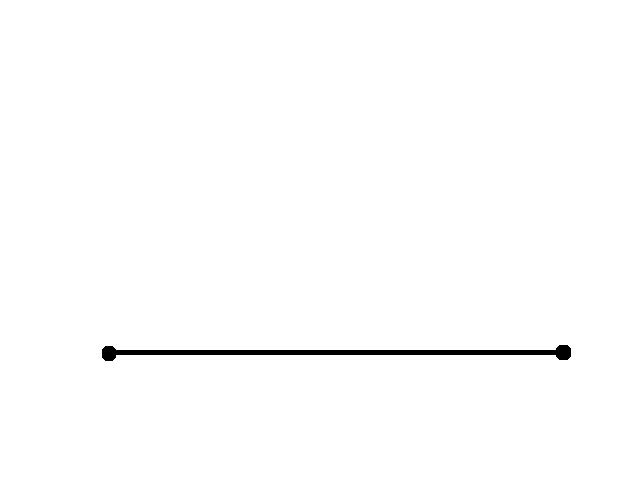
\includegraphics[height=2.25cm]{../Bilder/mpd_1.png}
  }
  \hspace{1cm}
  \subfloat[Kamal, Sarwar]{%
    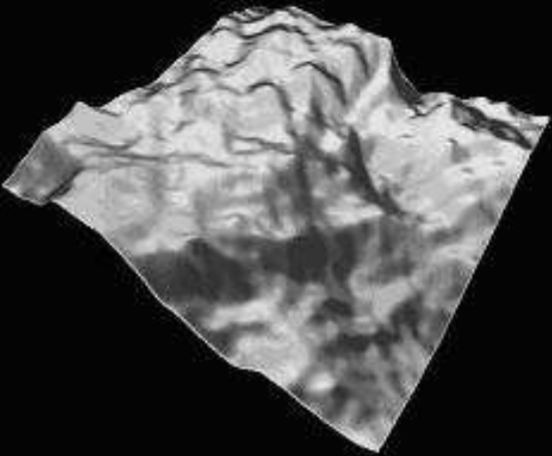
\includegraphics[height=2.25cm]{../Bilder/mpd.png}
  }
\end{figure}
}
\only<3>{
\begin{figure}[t]
  \subfloat[]{%
    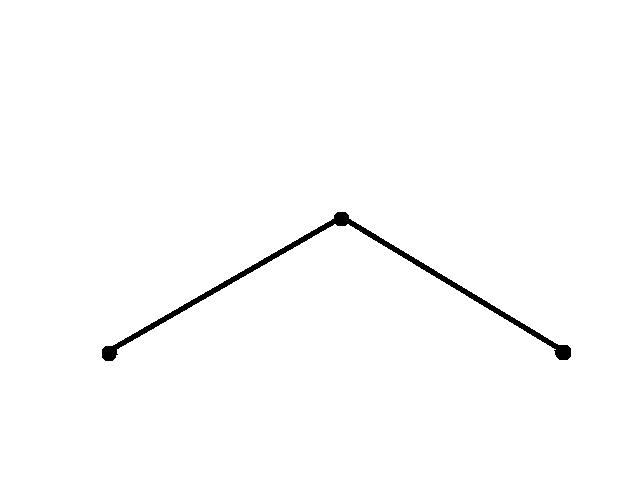
\includegraphics[height=2.25cm]{../Bilder/mpd_2.png}
  }
  \hspace{1cm}
  \subfloat[Kamal, Sarwar]{%
    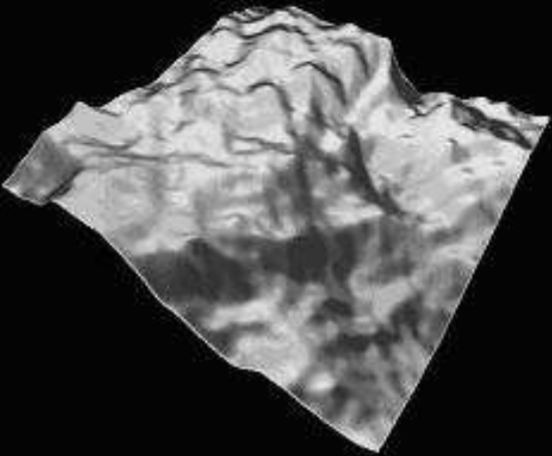
\includegraphics[height=2.25cm]{../Bilder/mpd.png}
  }
\end{figure}
}
\only<4>{
\begin{figure}[t]
  \subfloat[]{%
    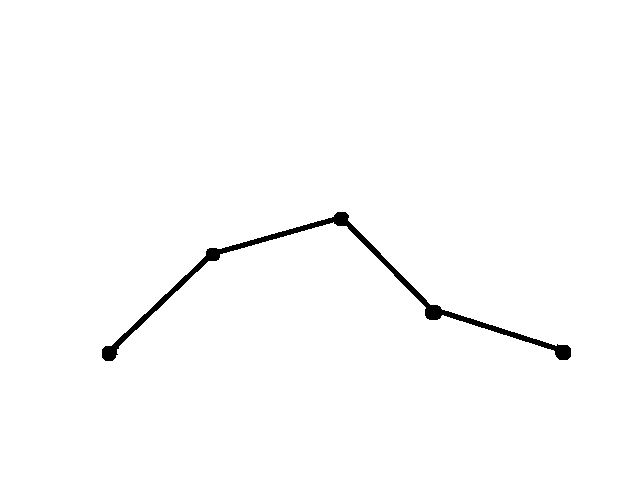
\includegraphics[height=2.25cm]{../Bilder/mpd_3.png}
  }
  \hspace{1cm}
  \subfloat[Kamal, Sarwar]{%
    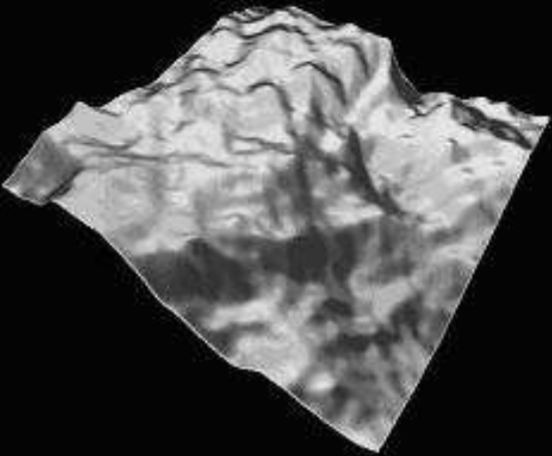
\includegraphics[height=2.25cm]{../Bilder/mpd.png}
  }
\end{figure}
}
\only<5>{
\begin{figure}[t]
  \subfloat[]{%
    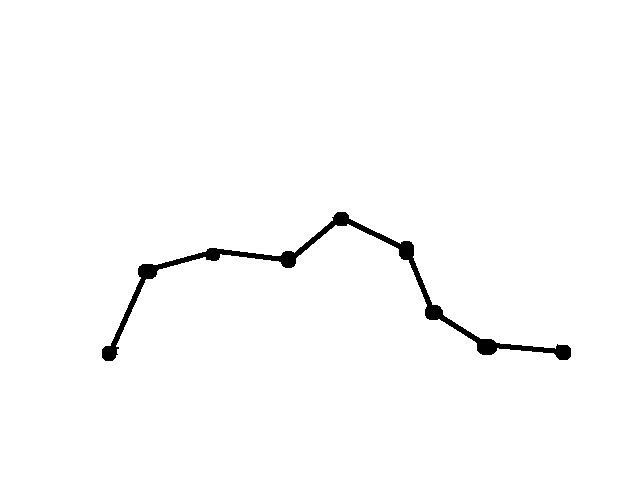
\includegraphics[height=2.25cm]{../Bilder/mpd_4.png}
  }
  \hspace{1cm}
  \subfloat[Kamal, Sarwar]{%
    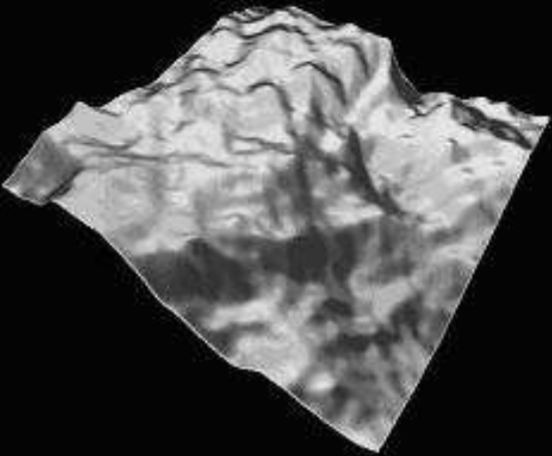
\includegraphics[height=2.25cm]{../Bilder/mpd.png}
  }
\end{figure}
}
\only<6>{
\begin{figure}[t]
\subfloat[Kamal, Sarwar]{%
  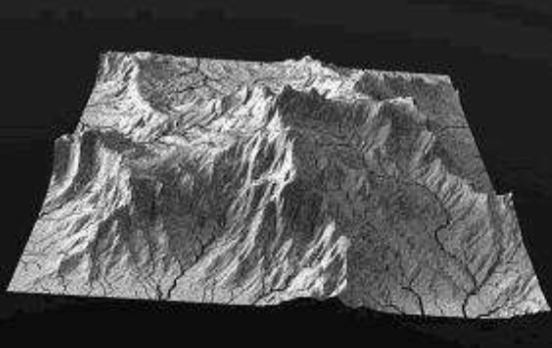
\includegraphics[height=3cm]{../Bilder/erosion.png}
}
\centering
\end{figure}
}
\only<7>{
\begin{figure}[t]
  \subfloat[lighthouse3d.com]{%
    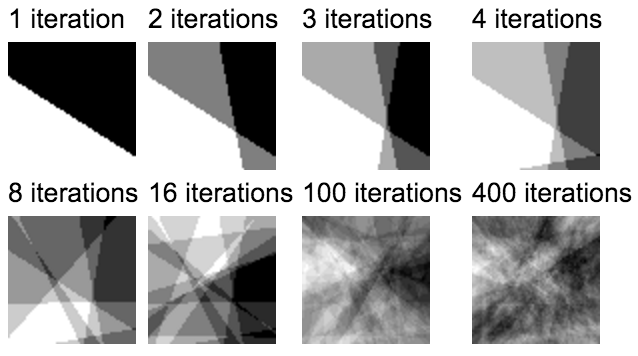
\includegraphics[height=2.5cm]{../Bilder/fault_1.png}
  }
  \hspace{1cm}
  \subfloat[Kamal, Sarwar]{%
    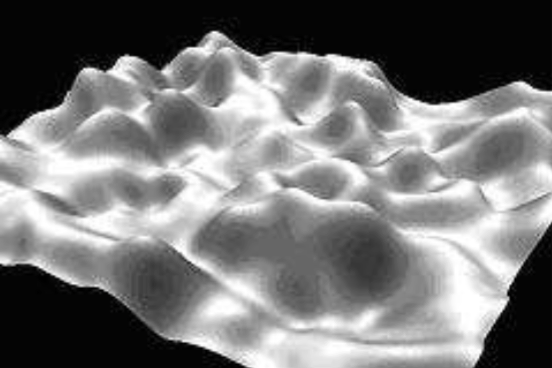
\includegraphics[height=2.5cm]{../Bilder/fault.png}
  }
\end{figure}
}
\only<8>{
\begin{figure}[t]
  \subfloat[Kamal, Sarwar]{%
    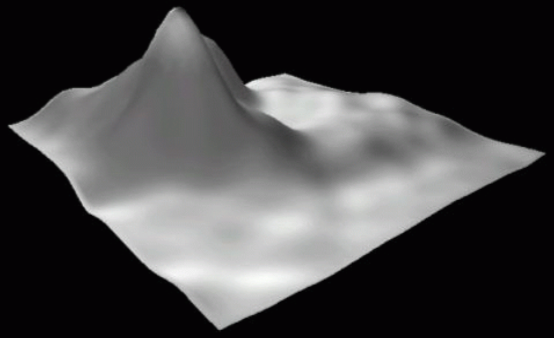
\includegraphics[height=3cm]{../Bilder/rmp.png}
  }
\end{figure}
}
\end{itemize}
\end{frame}

  \section{Geplante Herangehensweise}
  \frame{
    \frametitle{Geplante Herangehensweise}
    \begin{itemize}
      \item Testen diverser Algorithmen und abwägen ob es möglich ist diese anzupassen
      \item Erweitern des von Kamal und Sarwar vorgeschlagenen Algorithmus um ganze
        Gebirgsketten kontrolliert erzeugen zu können
      \begin{itemize}
        \item Verlauf,
        \item Höhe und
        \item Ausbreitung des Gebirges soll definierbar sein
      \end{itemize}
      \item Kombinieren vorgestellter Algorithmen zur Steigerung des Realismus
    \end{itemize}
  }

  \section*{Fragen?}
  \frame{
    \begin{center}
      \Huge Fragen?
    \end{center}
  }

\end{document}
